\documentclass[11pt]{article}
	
	%%%%%%%%%%%%%%%%%%%%%%%%%%%%%%%%%%%%%%%%%%%%%%%%%%%%%%%%%%%%%%%%%%%%%%
	%\pdfminorversion=4
	% NOTE: To produce blinded version, replace "0" with "1" below.
	\newcommand{\blind}{0}
	
	%%%%%%% IISE Transactions margin specifications %%%%%%%%%%%%%%%%%%%
	% DON'T change margins - should be 1 inch all around.
	\addtolength{\oddsidemargin}{-.5in}%
	\addtolength{\evensidemargin}{-.5in}%
	\addtolength{\textwidth}{1in}%
	\addtolength{\textheight}{1.3in}%
	\addtolength{\topmargin}{-.8in}%
    \makeatletter
    \renewcommand\section{\@startsection {section}{1}{\z@}%
                                       {-3.5ex \@plus -1ex \@minus -.2ex}%
                                       {2.3ex \@plus.2ex}%
                                       {\normalfont\fontfamily{phv}\fontsize{16}{19}\bfseries}}
    \renewcommand\subsection{\@startsection{subsection}{2}{\z@}%
                                         {-3.25ex\@plus -1ex \@minus -.2ex}%
                                         {1.5ex \@plus .2ex}%
                                         {\normalfont\fontfamily{phv}\fontsize{14}{17}\bfseries}}
    \renewcommand\subsubsection{\@startsection{subsubsection}{3}{\z@}%
                                        {-3.25ex\@plus -1ex \@minus -.2ex}%
                                         {1.5ex \@plus .2ex}%
                                         {\normalfont\normalsize\fontfamily{phv}\fontsize{14}{17}\selectfont}}
    \makeatother

	\usepackage{amsmath}
	\usepackage{graphicx}
	\usepackage{enumerate}
	\usepackage{natbib} %comment out if you do not have the package
	\usepackage{url} % not crucial - just used below for the URL
	
	\graphicspath{ {images/} }

	\begin{document}
		
	%%%%%%%%%%%%%%%%%%%%%%%%%%%%%%%%%%%%%%%%%%%%%%%%%%%%%%%%%%%%%%%%%%%%%%%%%%%%%%
	\def\spacingset#1{\renewcommand{\baselinestretch}%
		{#1}\small\normalsize} \spacingset{1}
	%%%%%%%%%%%%%%%%%%%%%%%%%%%%%%%%%%%%%%%%%%%%%%%%%%%%%%%%%%%%%%%%%%%%%%%%%%%%%%
		
    \title{Non Coding RNA in Growth Retardation}
    \author{BMI 5330 - Term Project \\
    Austin Vecchio \\
    Spring 2021 }
    \date{}
    \maketitle
		
		
	\begin{abstract}
This document provides a \LaTeX \ template for \emph{IISE Transactions}. Your paper should be compiled in the following order: title; abstract; keywords; main text, including an introduction and a conclusion or summary; acknowledgments; declaration of interest statement; references; appendices (as appropriate). Figures and tables should be inserted into the text as close to first mention as possible (NOT appended to the end of the manuscript). In-text citations and the reference list must follow \emph{IISE Transactions} guidelines. Use 11 point font, 1 inch margins, and double-spacing for the manuscript. A typical paper for this journal should be no more than 30 pages in manuscript format, counting from the title page to references. Appendices should be included as supplemental online materials. Do not use footnotes. \emph{IISE Transactions} uses a double-blind review process. Please make sure that you submit the \textbf{blind version} of your manuscript, which does not contain any information identifying the authors.  This includes removing the authors information on the title page as well as the information that may be identifying in the Acknowledgment section. We thank you for your attention to these details.
	\end{abstract}
			
	\noindent%
	{\it Keywords:} \emph{IISE Transactions}; \LaTeX; Manuscript format; Taylor \& Francis.

	%\newpage
	\spacingset{1.5} % DON'T change the spacing!


\section{Introduction and Background} \label{s:intro}


Growth Retardation is an uncommon disease where the development of tissues or organs improperly develop. One study (Boisell et al., 2009) describes the physical observations of eight toddlers known to have a genetic mutation. Several conditions of which these toddlers were diagnosed with include: hypertonicity or postnatal microcephaly in the central nervous system, hypertrophic cardiomyopathy in the cardiovascular system. Other conditions listed in Boisell et al., (2009) were described as growth malformations such as cutis marmorata, brachydactyly or an umbilical hernia. The variety and severity of conditions impacted the lifespan such that all diagnosed with Growth Retardation lived no longer than the age of three (Boisell et al., 2009). Another study (Çağlayan et al., 2016), described the observations and analyses regarding a single five year old female. This female similarly experienced a series of developmental issues which included seizures, respiratory issues and growth malformations such as an asymmetric skull (Çağlayan et al., 2016). Boisell et al., (2009) and Çağlayan et al., (2016) are two of many genome wide association studies conducted to have associated Growth Retardation to genetic mutations found in the Fat Mass and Obesity associated (FTO) gene. The FTO protein is tentatively classified as an AlkB dioxygenase (Ferenc et al., 2020). This primary function of protein with this classification is to repair alkylated DNA and RNA. Although the FTO protein has been observed to repair alkylated DNA and RNA, this task was rarely performed (Ferenc et al., 2020). Thus, the primary function of the FTO protein remains unknown. 

Genetic expression is a biochemical process for which a specified quantity of proteins are produced (Li et al., 2011) from a given gene such as FTO. In this process, RNA polymerase, binds to a promoter region in the DNA and is either strongly attracted to the promoter by an enhancer, or repelled by an insulator (Kolovos et al., 2012). The RNA polymerase transcribes specific regions of the DNA into messenger RNA (Li et al., 2011). Messenger RNA is then alternatively spliced into introns and exons by means of non coding RNA (Tazi et al., 2009). Only exons are fused in a specific order are to be translated into a chain of amino acids (Lam et al., 2021). The amino acid chain will fold in such a manner to form the resulting protein molecule (Dill et. Al, 1995). It has been described in literature such as Smith & Flodman (2018) that the genetic expression process can be disrupted by either mutations to the DNA. Disruptions in genetic expression result in either a variation in expression of the protein, or a non functional protein. 

Non coding RNA is classified as RNA that is not translated into protein (Gibb et al., 2011). There exist numerous types of non coding RNA that regulate messenger RNA or are involved in post transcriptional modifications steps of genetic expression. Non coding RNA are classified based on size and a generic set of functions. Described in Macfarlane & Murphy, (2010), MicroRNA is a short nucleotide sequence of ~20bp that assembles into a RNA-induced silencing complex. This complex targets a specific messenger RNA for which to regulate the amount produced (Macfarlane & Murphy, 2010). Circular RNA is the only closed loop RNA in which the 5’ and 3’ ends fuse to form a circular loop (Yu & Kuo, 2019). Circular RNA is formed from introns or exons that are a bi product of alternative splicing. The general function of Circular RNA involves interactions (transport/decoy) of microRNA (Yu & Kuo, 2019). Long non coding RNA (Gibb et al., 2011) is a generic classification of non coding RNA that encompasses other variety of non coding RNA such as lincRNA. Most forms of long non coding RNA either perform regulatory functions of messenger RNA, or are involved in enzymatic reactions (Gibb et al., 2011). The individual functions of these RNAs are determined by both structure (secondary/tertiary) and structural components. Some examples of structural components in ncRNA include hairpins, stems, multi loops, and interior loops (Zampetaki et al., 2018). Examples of these structures can be viewedin Figure 1. 

\begin{figure}[t]
	\centering
	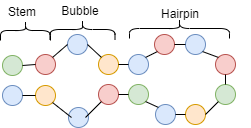
\includegraphics[width=8cm]{rna-struct}
	\caption{A diagram of the following non coding RNA structural components: stem, bubble hairpin.
	}
	\label{fig:mesh1}
\end{figure}

If any process within the expression of a gene is disrupted, an irregular amount of protein would be produced. This undesirable behavior would result in some form of illness. Two studies performed discovered that dysfunctional non coding RNA resulted in disease. The first study performed by Zhou & Li (2021) was an investigation into Hereditary Kidney Disorders that discovered mutations in either the PKD1 or PKD2 genes. These mutations alter the functionality in either long non coding RNA or microRNA (Zhou & Li, 2021). Thereby, these kidney disorders are a result of destructive behavior within the cell originating from these dysfunctional non coding RNA. Some examples reported in Zhou & Li (2021), describe the negative impact of these non coding RNA which includes the repression of expressing the PKD1 or PKD2 gene, defects in the mitochondrial metabolism or in severe circumstances, bring about apoptosis. The second study was a systematic review by Xu et al. (2021) for literature involving the dysregulation of extracellular vesicles that transport non coding RNA between cells. In this review, the authors amassed evidence of dysfunctional RNA resulting in neurodegenerative disorders. It was found that Long non coding RNAs were attributed to Parkinsons Disease, and both circular RNA and microRNA were linked to Alzheimer's disease (Xu et al., 2021). The results of the investigation found that dysfunctional Long non coding RNA, micro RNA or circular RNA that is transported via extra cellular vesicles are damaging to the cell such in such a manner as to cause neuro degenerative diseases (Xu et al., 2021). Thus, there exists significant experimental evidence of dysfunctional non coding RNA resulting in disease.  

In 2018, a study by Giral & Kratzer (2018) examined the frequency of genome wide associated variants occurring within locations of interest within the gene. This analysis leveraged the NHGRI-EBI and GWASdb.v2 databases as these catalogs provide associations to a genomic region (enhancer, circRNA, promoter, exon) of which the variant occurs within. In this investigation, Giral & Kratzer (2018) reported that a significant majority (90%) of disease associated variants exist outside of coding regions. This implies that most diseases are due to improper expression of proteins compared to malformed protein structures. Although this discovery may alter the approach to understanding genetic expression and disease, the significant finding reported by this investigation was that 45% of all disease associated variants occur within long non coding RNA (Giral & Kratzer, 2018).   

 

The available public literature for the impact of variants in non coding RNA structure is sparse. Although, there exists significant research performed on the structural formation of non coding RNAs. For all types of non coding RNA, the structures are formed through the hydrogen bonding of nucleotides (Chillón & Marcia, 2020). Although it can be theorized as to the effects of altering a single nucleotide sequence, the actual effects of such a change could produce a variety of alterations to either the overall structure or individual structural components. In protein, the degree of structural change to the resulting protein is dependent on if the variation is an insertion/deletion or a single nucleotide polymorphism (Feyfant, Sali & Fiser, 2007). An insertion or deletion can produce cascading effects that is certain to negatively affect the resulting structure, or a single nucleotide polymorphism would alter only one amino acid within the chain (Feyfant, Sali & Fiser, 2007). The altered amino acid may yield significant or insignificant structural changes to the resulting protein. To understand how dysfunctional non coding RNA results in a condition, the structural variation, including variation of components would warrant analysis. 

With the increasing evidence of dysfunctional non coding RNA in disease, there was significant interest in exploring the association of non coding RNA within Growth Retardation and further the understanding for how dysfunctional RNA may result in Growth Retardation. To accomplish this, a series of public data sets were leveraged to perform both frequency analyses for variants intersecting non coding RNA and a set of analyses of structural variation for associated non coding RNA. 

\section{Methods and Datasets} \label{s:methods}

 

All data retrieval, operations and analyses were conducted through a python script (v 3.8.5). The script, all utilities and documentation are stored in a source code repository. All data can be viewed from a cloud hosted file share. The locations of the source code and the data are found within the Supplemental section of this article. All experimentally verified variants and genomic regions were acquired from several databases which are listed in Table 1. The programmatical method for retrieving the data either involved Api requests, file downloads or database (SQL) queries. Data obtained by SQL query or Api request are cached as a json file on the local directory. Genomic regions other than transcript regions such as coding sequences (CDS) or untranslated regions (UTR 3’, UTR 5’) and non coding RNA were include in the event that Growth Retardation variants were associated with an unexpected region (enhancer, insulator). 

\begin{figure}[t]
	\centering
	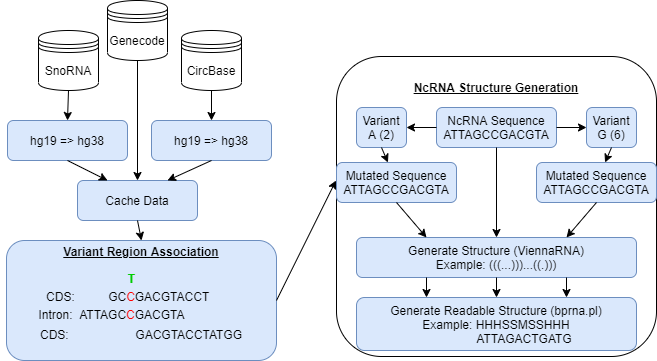
\includegraphics[width=8cm]{workflow}
	\caption{A diagram depicting the high level workflow of the python script used for the analysis.
	}
	\label{fig:mesh1}
\end{figure}

Several databases stored coordinate data for genomic regions or variants in the hg19 coordinate format. The current version of the human genome coordinate system is hg38. As a result, the coordinate systems for data sets retrieved from databases using the hg19 format were translated into the hg38 format via the LiftOver python package. The human genome coordinate format for each database is listed in Table 1. 

The GENECODE annotations provides coordinate data for exons, coding sequences (CDS), and both untranslated regions (UTR 3’, UTR 5’). To extract the coordinate data of the introns, the Bedtools software (Quinlan & Hall, 2010) suite was leveraged in a two step method that is displayed in Figure 2. The coordinates for overlapping exons are initially merged. Then, the coordinates for the gaps between merged exons were calculated. These gapped coordinates represent the introns existing within the transcripts. Exons were not included in the analysis as exons are comprised of CDS, UTR 3’ and UTR 5’ regions. The inclusion of CDS, UTR 3’ and UTR 5’ regions were included in favor to provide additional granularity for the frequency analyses. 

\begin{figure}[t]
	\centering
	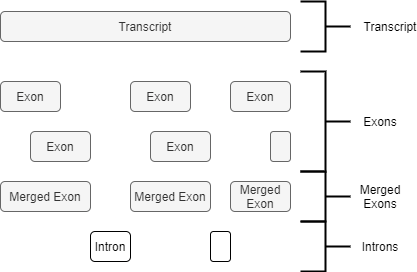
\includegraphics[width=8cm]{bed-tools}
	\caption{A diagram exhibiting BedTool processes used to extract intron coordinates from known exon and transcript coordinates.
	}
	\label{fig:mesh1}
\end{figure}

Circular RNA databases, including CircBase stores only a single coordinate set (start and end position) which includes all spliced sequences found within the DNA in addition to extraneous genomic information. The sub coordinates of circular RNA which represents introns and exons that are a bi product of alternative splicing were obtained through an algorithmic process that is displayed in Figure 3. For this process, the Longest Common Subsequence algorithm locates a shared genomic sequence that exists in both the inclusive genomic sequence and the corresponding consensus RNA sequence provided by CircBase. The coordinates for this sequence are obtained and transformed to reflect the absolute coordinate found within the hg38 coordinate system. The shared sequence in the consensus RNA sequence is then replaced by a marker. This process is repeated until only markers remain. This process generates a set of sub coordinates of the introns and exons used to construct the representative circular RNA. The sub coordinate sets are then reindexed by means of the resulting markers to ensure proper ordering when reconstructing the consensus string for the structural analysis. 


\begin{figure}[t]
	\centering
	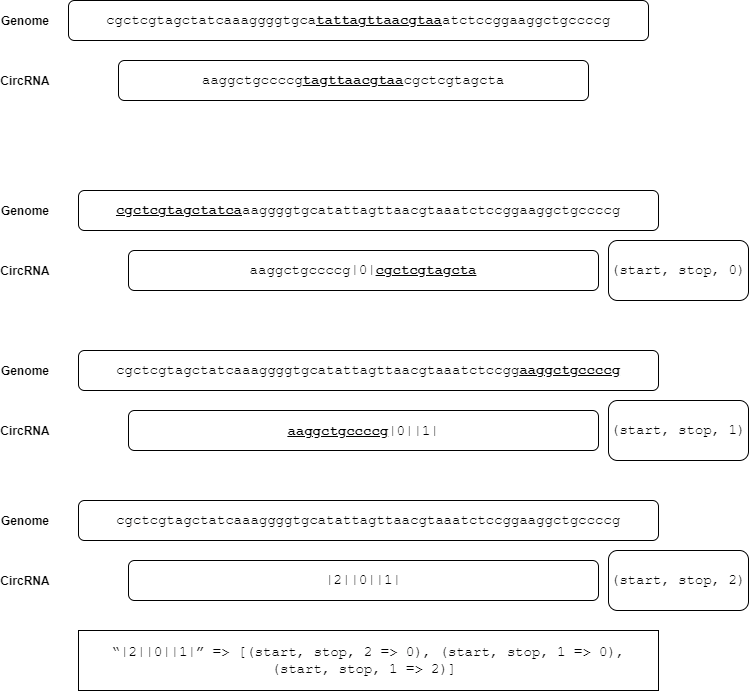
\includegraphics[width=8cm]{circrna-algorithm}
	\caption{An workflow of steps for extracting the sub coordinates of circular RNA by means of the longest common subsequence algorithm.}
	\label{fig:mesh1}
\end{figure}

After obtaining all Growth Retardation variants and genomic regions of interest, variants were then associated to genomic regions by coordinates. The association occurs under the condition that the variants start or end position was within, and includes, the defined start and end position for the genomic region. These associated data sets were analyzed through a set of frequency analyses. 

An initial analysis of these associations evaluated the frequency of variants within occurring within genomic regions to measure the concentration of variants intersecting a type of genomic region. With potential overlap of genomic regions, it is plausible for frequencies in this analysis to be inflated as variants would be tallied for multiple occurrences. Therefore, two additional analyses were performed to measure both the number of genomic regions and number of genomic region types intersected by these variants. To observe non coding specific variants, a specific frequency association was performed to measure the number of Growth Retardation variants that intersect non coding RNA regions and not intersect coding sequences. Under random occurrence, variants should be distributed based on the proportion of genomic coverage for a region type (enhancer, CDS). A chi square test was performed to statistically evaluate if there exists a diversion from the expected random occurrence distribution.  

The structures for all non coding RNAs and associated variants were generated in a multi step process orchestrated by the python script. For this process, each variant existing within the non coding RNA was applied to the sequence such that a mutant sequence was generated. The structures for all non coding RNA sequences and mutant sequences were generated by means of the ViennaRNA software suite (Lorenz et al., 2011). In the post processing step, the Perl script, bpRNA.pl (Danaee et. Al, 2018) transformed the structural output of ViennaRNA into a format for which could be analyzed.  

An initial structural analysis measured the frequency of a structural component occurring within all non coding RNA reference structures compared to all mutant structures. A second structural analysis was performed to measure the deviation in orientation of the mutated structure compared to the associated non coding RNA reference structure. A string differential algorithm was applied to generate a list of modifications required to transform the reference structural string into the mutated structural string. A percent change to the reference structural string was calculated using the quantity of modifications produced by the string differential operation.  

\begin{figure}[t]
	\centering
	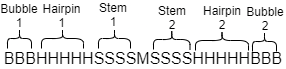
\includegraphics[width=8cm]{struct-freq}
	\caption{A diagram depicting an example of an RNA structural string and how structural components are counted from this string.
	}
	\label{fig:mesh1}
\end{figure}

\begin{figure}[t]
	\centering
	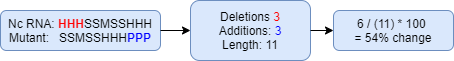
\includegraphics[width=8cm]{diff-process}
	\caption{A high level overview of the algorithmic process to determine the percent difference of two RNA structural strings.
	}
	\label{fig:mesh1}
\end{figure}

\section{Results} \label{s:results}

\subsection{
\emph{Data}} \label{s:conclusion}

The database search results for Growth Retardation variants and regions associated with the FTO gene can be viewed in Table 1. The FTO gene consists of 23 transcripts which contains 145 unique exons and 50 shared intronic regions. The FTO gene contains a single promoter, 6 insulators and 107 enhancers. The quantity of enhancers obtained is due to the inclusion of enhancers from all tissue types. Only two types of non coding RNA are found within the FTO gene. There are 19 circular RNA and 19 long non coding RNA. 


    \begin{table}[!hbt]
      % Center the table
      \begin{center}
      % Fold Inductions
      \caption{QtPCR Fold Inductions}
      \label{tab:simParameters}
      % Table itself: here we have two columns which are centered and have lines to the left, right and in the middle: |c|c|
      \begin{tabular}{|c|c|c|}
        \hline
		Database           & Data Type(s) & Result(s) \\
        \hline
		GWAS Catalog & Variant & 0 \\
        \hline
		ClinVar & Variant & 117 \\
        \hline
		Genecode & CDS, UTR 3, UTR 5  & 109, 27, 16  \\
        \hline
		Genecode & Exon (not used), Intron  & 145, 50 \\
        \hline
		RNACentral & NcRNA  & 19 \\
        \hline
		CircBase & CircRNA  & 19 \\
        \hline
		SnoDB & SnoRNA  & 0 \\
        \hline
		Eukaryotic Promoter Db & Promoter & 1 \\
        \hline
		Enhancer Atlas & Enhancer & 107 \\
        \hline
		CTCFBSDB & Insulator & 0 \\
        \hline
      \end{tabular}
      \end{center}
    \end{table}

\subsection{
\emph{Freq Analysis}} \label{s:conclusion}

\subsubsection{\emph{Sub-subsection heading 3.1.1}} \label{s:methods.1.1}

Table 2 in Appendix E displays the frequency for variants occurring within specific region types. It was found that no variants related to Growth Retardation occur within the enhancers, insulators or long non coding RNA. Seen in Figure 4, there exists a concentration (97%) of variants within CDS, UTR 3’ and circular RNA regions. All other regions exhibit at least one Growth Retardation variant.  

\begin{figure}[t]
	\centering
	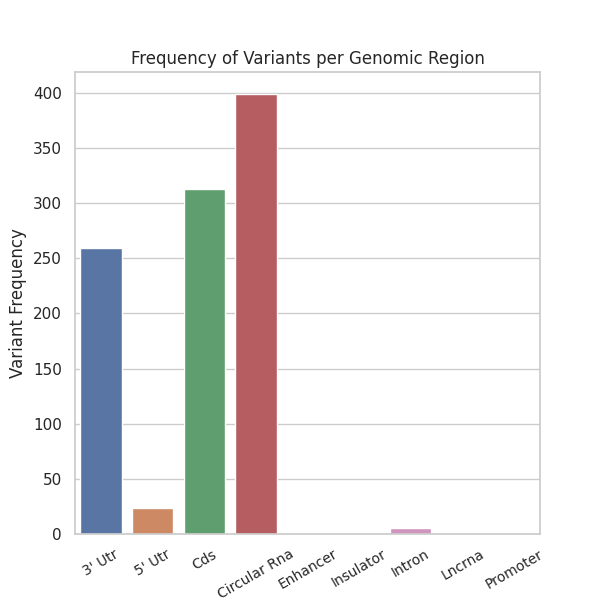
\includegraphics[width=8cm]{variant_frequencies}
	\caption{The frequency of variants within types of genomic regions.
	}
	\label{fig:mesh1}
\end{figure}

\subsubsection{\emph{Sub-subsection heading 3.1.1}} \label{s:methods.1.1}

The frequency of a variants within genomic region types is displayed in Figure 4. It was found that 17% of the variants impact three regional types, 71% of variants impacts two regional types and only 12% of variants impact only a single region type. The frequency of variants intersecting with two or three types of genomic regions correlates to the original frequency graph. The frequency analysis results for the number of regions for which variants intersect is displayed in Figure 5. The highest frequencies  of variants were found to intersect 2, 3, 6, and 7 genomic regions. This displays a significant level of overlap of genomic regions within the FTO gene.  

\begin{figure}[t]
	\centering
	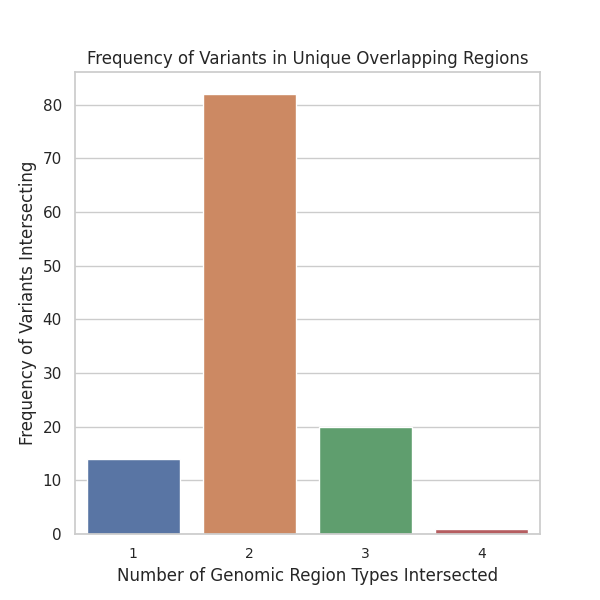
\includegraphics[width=8cm]{unique_non_overlap_variants}
	\caption{The frequency of variants intersecting a certain quantity of genomic regions. These regions could be of the same type.
	}
	\label{fig:mesh1}
\end{figure}

\begin{figure}[t]
	\centering
	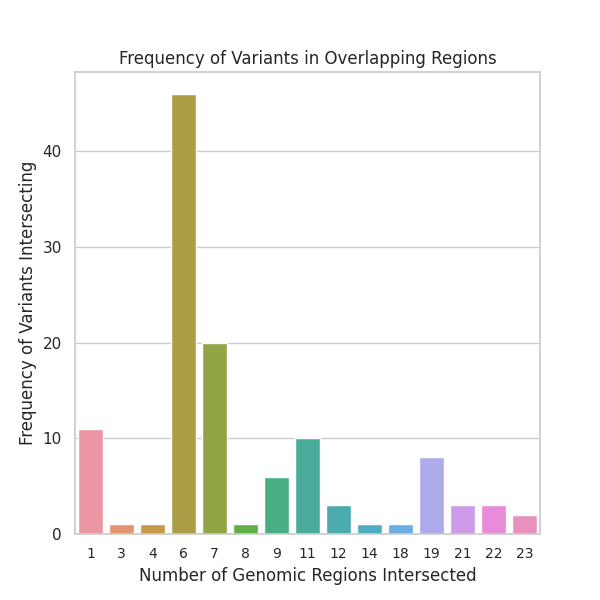
\includegraphics[width=8cm]{unique_overlap_variants}
	\caption{The frequency of variants intersecting a certain quantity of genomic region types.
	}
	\label{fig:mesh1}
\end{figure}

\subsubsection{\emph{Sub-subsection heading 3.1.1}} \label{s:methods.1.1}

The expected distribution of the variants anticipates 1.4% of variants within circular RNA, 11.7% of variants within enhancers, 0.4% of variants in coding regions, and 7% of variants within long non coding RNA. The results of the chi-square test revealed that the observed distribution of Growth Retardation variants among regions differed significantly from the expected distribution (Df=8, p > 0.0001). Of the observed concentration of variants and genomic regions, a total of 66 of the 117 Growth Retardation variants were found to intersect circular RNA and not the coding sequences. 

	\begin{table}[!hbt]
      % Center the table
      \begin{center}
      % Fold Inductions
      \caption{QtPCR Fold Inductions}
      \label{tab:simParameters}
      % Table itself: here we have two columns which are centered and have lines to the left, right and in the middle: |c|c|
      \begin{tabular}{|c|c|c|c|c|}
        \hline
		Genomic Region & Actual & Expected \\
        \hline
        Insulator & 0 & 8 \\
        \hline
        Enhancer & 0 & 118 \\
        \hline
        Coding Sequences & 313 & 4 \\
        \hline
        UTR 3 & 259 & 28 \\
        \hline
        UTR 5 & 24 & 1 \\
        \hline
        Intron & 5 & 755 \\
        \hline
        Promoter & 1 & 0 \\
        \hline
        Long Non Coding RNA & 0 & 71 \\
        \hline
        Circular RNA & 399 & 14 \\
        \hline
      \end{tabular}
      \end{center}
    \end{table}

\subsection{
\emph{Struct Analysis}} \label{s:conclusion}

\subsubsection{\emph{Sub-subsection heading 3.1.1}} \label{s:methods.1.1}

Figure 4 displays the structural component analysis comparing structural frequencies within all non coding RNA reference structures to mutant structures. It was found that all structural components are significantly more frequent in mutant structures compared to the reference ncRNA structures. Only unpaired regions and segments are uninterpretable due to the infrequent occurrences of these structures within circular RNA.  

\begin{figure}[t]
	\centering
	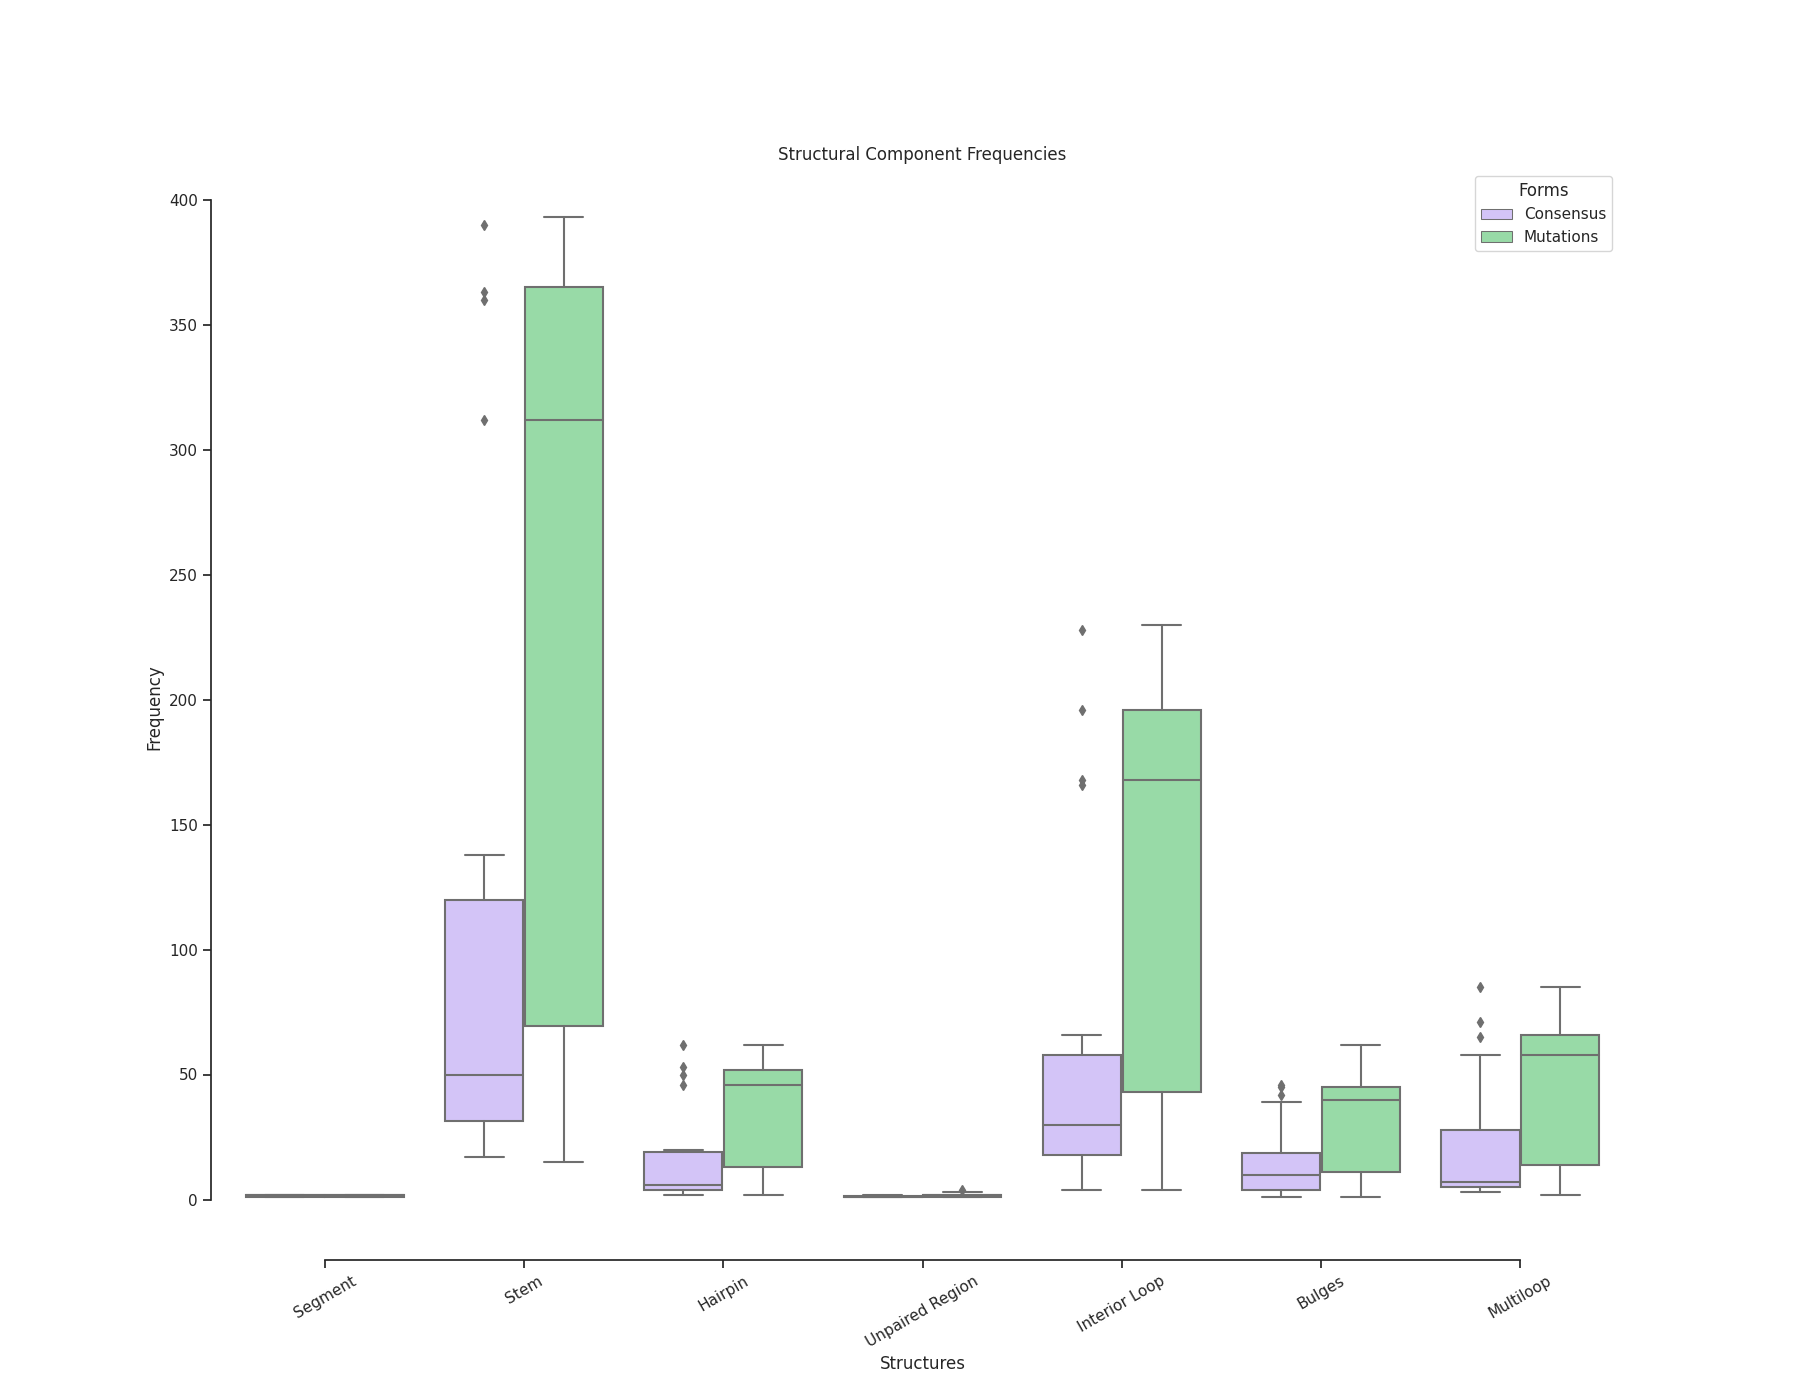
\includegraphics[width=8cm]{boxes}
	\caption{Grouped boxplots of the frequency of structural components within all reference structures compared to mutated structures.
	}
	\label{fig:mesh1}
\end{figure}

\subsubsection{\emph{Sub-subsection heading 3.1.1}} \label{s:methods.1.1}

The analysis of difference in structural orientation between mutated structures and associated reference structures displayed a wide range of frequencies in percent differences. Nearly half (45%) of the structural differences exhibited less than 10% of structural changes. 54% of mutated structures differed from the reference structure by more than 20%. One third of all structural changes exhibited a significant degree of structural differences (>90%) in comparison to the reference structures.  

\begin{figure}[t]
	\centering
	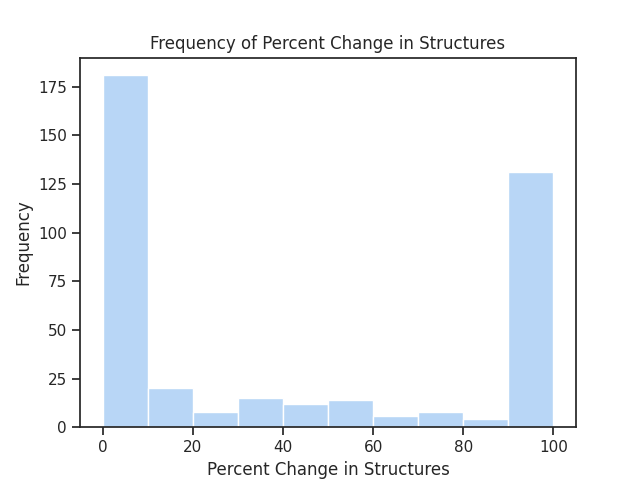
\includegraphics[width=8cm]{structs}
	\caption{A histogram of the percent differences between variant non coding RNA structures and associated reference RNA non coding RNA structures.
	}
	\label{fig:mesh1}
\end{figure}

\section{Discussion} \label{s:discussion}


\subsection{
\emph{Freq Analysis}} \label{s:conclusion}

The chi square test confirmed that the frequencies of variants occurring in genomic regions differed from the expected distribution. The expected distribution of variants was dependent on the coverage of each region type within the FTO gene. Therefore, the higher coverage of a region should yield a higher quantity of variants under the condition the variants were randomly dispersed. The observed distribution was that a concentration of Growth Retardation variants occurred within circular RNA, UTR 3’, UTR 5’ and CDS regions. Although few variants linked to Growth Retardation were found in the promoter and introns, it was unusual for no variants to occur within the enhancers, insulators, or long non coding RNA. This observation suggests that variation to either the circular RNA or the resulting protein structure for the FTO gene would result in Growth Retardation. Although not pertinent to this investigation, the inclusion of additional genomic regions provided additional insight in that variation of the promoter would also yield Growth Retardation.  

The frequency analysis of variants in genomic regions displayed frequencies within the CDS, UTR 3’ and UTR 5’ that exceed the quantity of Growth Retardations obtained. Therefore, there exists some degree of overlap between these three regions. As frequency analyses construct observations from a singular viewpoint, additional frequency analyses must be constructed. This is a known limitation of this approach. Therefore, to explore the high frequencies in the CDS, UTR 3’ and UTR 5’ regions, two additional frequency analyses were conducted to observe variants intersecting overlapping genomic regions. The number of genomic regions intersected by variants as seen in Figure 1 displays a significant degree of overlap with a majority of variants intersecting 3 to 7 genomic regions. This observation would explain the high frequencies recorded for the analysis of variants occurring within genomic regions as there may exist multiple regions of the same type intersected by a single variant. Therefore, the variant would be counted multiple times for a single genomic region type.  

The frequency analysis for variants intersecting unique genomic region types revealed a majority of variants impacted two or three genomic region types. Although this analysis masks the types of genomic regions for which are intersected, used in conjunction with the genomic region frequency analysis, an interpretation can still be conducted. The data presented for the variants intersecting unique genomic region types corresponds to the frequency analysis of variants occurring in genomic regions where most variants occurred within three types of genomic regions. This analysis further supports the high degree of overlap that was observed such that the untranslated regions, coding sequences and circular RNA occur within the same genomic range. The overlap of circular RNA is not unusual as circular is composed of introns and exon bi products from alternative splicing. Although variants intersecting multiple genomic regions could increase the disruption within genetic expression and may yield additional undesirable effects. While all three of these frequency analysis provide singular viewpoints upon which to view this data, the culmination of these frequency analysis on this data supplemented for the usage of a genome browser.  

Growth Retardation variants found within the coding sequences would result in altered protein structure. The effects of which would disable or weaken the functionality of the protein. Therefore, the effects of variants intersecting both CDS and circular RNA regions could in theory be masked. Due to the significant overlap occurring between transcripts and circular RNA, a final calculation performed. In discovering that 66 of 117 Growth Retardation variants occur within circular RNA regions and not in coding sequences suggests the hypothesis for which dysfunctional circular RNA in the FTO gene results in Growth Retardation. 

 

\subsection{
\emph{Struct Analysis}} \label{s:conclusion}

The comparison of the average frequency of structural components in mutated structures against reference ncRNA structures exhibited an unexpected pattern. The average of structural components in mutated structures was significantly higher compared to the reference structures. This pattern was observed in all comparisons for types of structural components within circular RNA. Although this analysis demonstrates a degree structural impact induced by variants, the degree for which the structure and structural components alter is not fully exhibited. This is a result of grouping all reference structures and mutant structures into a single group. In addition, due to the nature of the data set, there exists some skepticism for potentially inflated values as there exists more mutant structures compared to reference structures. Although this information presents indicators of significant structural changes, an alternative analysis was performed. 

The second structural analysis was conducted to further evaluate structural modifications to circular RNA as a result of variation. It was unexpected for a majority of the structural changes to either be significant (>90% diff) or insignificant (<10% diff). Structural alterations between 10% and 90% were infrequent in comparison. Although the variant data set contained several indels, a majority of the variants were single nucleotide polymorphisms. While the high frequency of significant structural changes (>40%) are most likely due to several of the 10 indels that occur within the FTO gene. It is plausible for a portion of these significant structural alterations within the non coding RNA structure to be a result of single nucleotide polymorphisms which would signify some form of sensitivity of structural formation. The structures that underwent significant structural changes (>90% diff) as a result of variation are predicted to either have some degree in loss of functionality or altered functionality such that the malformed non coding RNA would negatively impact components within the cell. Studies such as Zhou & Li (2021) or Xu et al. (2021) would suggest the structures exhibiting severe structural differences (>40%) would either be non functional or conduct a different set of undesired operations. For the minor structural changes observed, there does exist the situation for which variation occurs within the enzymatic (hairpin) components of the circular RNA  for which some functionality is lost. Determining loss of enzymatic functionality or minor structural changes would require additional analysis either by means of overlapping structural comparison or by means of a wet lab experiment. 

Both structural analyses were based on all variants intersecting with non coding RNA, and therefore includes variants also intersecting with coding sequences. These analyses were intended to analyze the degree of structural changes as a result of variants. To observe the structural alterations of non coding RNA that directly result in Growth Retardation, an additional analysis would need to be performed. The inclusion of this additional analysis was an initial oversight in the design of this project and was not able to be performed due to time constraints. 

\subsection{
\emph{Conclusion}} \label{s:conclusion}

The significant degree of structural change as a result of the variations to occur within half of the circular RNA would either disable or alter the functionality to a degree as to negatively impact the genetic expression of the FTO gene and possibly other components within the cell. The high frequency of significant structural changes in circular RNA coupled with the majority of Growth Retardations existing outside of coding sequences and within circular RNA presents significant evidence for which dysfunctional circular RNA would result in Growth Retardation. Although given this significant evidence, the hypothesis of dysfunctional non coding RNA resulting in Growth Retardation would require experimental verification to confirm and further explore the findings within this analysis. 
\subsection{
\emph{Proposal Differential}} \label{s:prop differential}

In the endeavor for conducting a series of scientific analyses originally defined in the proposal, there were several deviations conducted to obtain the necessary data and results. These deviations were due to a lack of experience within the bioinformatics field and general knowledge regarding the available data. The deviations to the proposal are briefly outlined in the following paragraphs. 

Minor adjustments were made to the databases queried. The SnoRNA database (snoDB) was added to the analysis after the proposal once realized that RNA central did not include snoRNA data. The proposed insulator database was exchanged for CTCFBSDB 2.0 due to the availability of data. Although the original proposed database allowed for the data sets to be downloaded, the download process could only be conducted manually. In favor of constructing a script to streamline the data acquisition process, the CTCFBSDB 2.0 database was utilized instead. 

It was not originally known of the existence of multiple coordinate systems within the human genome. Therefore, the coordinates needed to be adjusted with the LiftOver package. The absence of introns provided by GENECODE prompted the usage of bedtools in order to derive the coordinate data of the introns from the available exon coordinates. The absence of sub coordinates provided by CircBase presented an issue of accuracy. This was initially overlooked due to the unknown nature of circular RNA and the improper examination of data recorded in the database. Therefore, a computational method (outlined in the methods section) was constructed to determine the sub coordinates of the circular RNA. 

It was not expected for the large degree of overlap between genomic regions. As a result, two additional frequency analyses were constructed to measure variants intersecting overlapping genomic regions. A meaningful conclusion could not be performed from the initial structural analysis. Therefore, a second analysis was performed such that meaningful interpretations in the structural transformations could be measured. These analyses, although provided useful information, do not specifically examine variants that occur only within non coding RNA. This was realized after thorough examination of the data of which the adjustment to these analyses could not be met due to time constraints. 

There were several operational deviations due to time constraints. This includes not making code commits in the manner described in the proposal. In addition, there exist far fewer unit tests then what was proposed. Although all code is operational, the organization of the code could use improvements.

\section{References} \label{s:references}

Boissel, S., Reish, O., Proulx, K., Kawagoe-Takaki, H., Sedgwick, B., Yeo, G. S., Meyre, D., Golzio, C., Molinari, F., Kadhom, N., Etchevers, H. C., Saudek, V., Farooqi, I. S., Froguel, P., Lindahl, T., O'Rahilly, S., Munnich, A., & Colleaux, L. (2009). Loss-of-function mutation in the dioxygenase-encoding FTO gene causes severe growth retardation and multiple malformations. American journal of human genetics, 85(1), 106–111. https://doi.org/10.1016/j.ajhg.2009.06.002 

Çağlayan, A., Tüysüz, B., Coşkun, S. et al. A patient with a novel homozygous missense mutation in FTO and concomitant nonsense mutation in CETP. J Hum Genet 61, 395–403 (2016). https://doi.org/10.1038/jhg.2015.160 

Chillón, I., & Marcia, M. (2020). The molecular structure of long non-coding RNAs: emerging patterns and functional implications. Critical reviews in biochemistry and molecular biology, 55(6), 662–690. https://doi.org/10.1080/10409238.2020.1828259 

Danaee, P., Rouches, M., Wiley, M., Deng, D., Huang, L., & Hendrix, D. (2018). bpRNA: large-scale automated annotation and analysis of RNA secondary structure. Nucleic acids research, 46(11), 5381–5394. https://doi.org/10.1093/nar/gky285 

Dill, K. A., Bromberg, S., Yue, K., Fiebig, K. M., Yee, D. P., Thomas, P. D., & Chan, H. S. (1995). Principles of protein folding--a perspective from simple exact models. Protein science : a publication of the Protein Society, 4(4), 561–602. https://doi.org/10.1002/pro.5560040401 

Ferenc, K., Pilžys, T., Garbicz, D. et al. Intracellular and tissue specific expression of FTO protein in pig: changes with age, energy intake and metabolic status. Sci Rep 10, 13029 (2020). https://doi.org/10.1038/s41598-020-69856-5 

Feyfant, E., Sali, A., & Fiser, A. (2007). Modeling mutations in protein structures. Protein science : a publication of the Protein Society, 16(9), 2030–2041. https://doi.org/10.1110/ps.072855507 

Gao, Xue & Shin, Yonghyun & Wang, Fei & Tong, Qiang & Zhang, Pumin. (2010). The Fat Mass and Obesity Associated Gene FTO Functions in the Brain to Regulate Postnatal Growth in Mice. PloS one. 5. e14005. 10.1371/journal.pone.0014005. 

Gibb, E.A., Brown, C.J. & Lam, W.L. The functional role of long non-coding RNA in human carcinomas. Mol Cancer 10, 38 (2011). https://doi.org/10.1186/1476-4598-10-38 

Giral, H., Landmesser, U., & Kratzer, A. (2018). Into the Wild: GWAS Exploration of Non-coding  RNAs. Frontiers in cardiovascular medicine, 5, 181.  https://doi.org/10.3389/fcvm.2018.00181 

Kolovos, P., Knoch, T. A., Grosveld, F. G., Cook, P. R., & Papantonis, A. (2012). Enhancers and silencers: an integrated and simple model for their function. Epigenetics & chromatin, 5(1), 1. https://doi.org/10.1186/1756-8935-5-1 

Lam, S. D., Babu, M. M., Lees, J., & Orengo, C. A. (2021). Biological impact of mutually exclusive exon switching. PLoS computational biology, 17(3), e1008708. https://doi.org/10.1371/journal.pcbi.1008708 

Li, G. W., & Xie, X. S. (2011). Central dogma at the single-molecule level in living cells. Nature, 475(7356), 308–315. https://doi.org/10.1038/nature10315 

Lorenz, R., Bernhart, S. H., Höner Zu Siederdissen, C., Tafer, H., Flamm, C., Stadler, P. F., & Hofacker, I. L. (2011). ViennaRNA Package 2.0. Algorithms for molecular biology : AMB, 6, 26. https://doi.org/10.1186/1748-7188-6-26 

Macfarlane, L. A., & Murphy, P. R. (2010). MicroRNA: Biogenesis, Function and Role in Cancer. Current genomics, 11(7), 537–561. https://doi.org/10.2174/138920210793175895 

Quinlan, A. R., & Hall, I. M. (2010). BEDTools: a flexible suite of utilities for comparing genomic features. Bioinformatics (Oxford, England), 26(6), 841–842. https://doi.org/10.1093/bioinformatics/btq033 

Rohena, L., Lawson, M., Guzman, E., Ganapathi, M., Cho, M. T., Haverfield, E., & Anyane-Yeboa, K. (2016). FTO variant associated with malformation syndrome. American journal of medical genetics. Part A, 170A(4), 1023–1028. https://doi.org/10.1002/ajmg.a.37515 

Smith, M., & Flodman, P. L. (2018). Expanded Insights Into Mechanisms of Gene Expression and Disease Related Disruptions. Frontiers in molecular biosciences, 5, 101. https://doi.org/10.3389/fmolb.2018.00101 

Tazi, J., Bakkour, N., & Stamm, S. (2009). Alternative splicing and disease. Biochimica et biophysica acta, 1792(1), 14–26. https://doi.org/10.1016/j.bbadis.2008.09.017 

Xu, Y. Z., Cheng, M. G., Wang, X., & Hu, Y. (2021). The emerging role of non-coding RNAs from extracellular vesicles in Alzheimer's disease. Journal of integrative neuroscience, 20(1), 239–245. https://doi.org/10.31083/j.jin.2021.01.360 

Yeo, G. S., & O'Rahilly, S. (2012). Uncovering the biology of FTO. Molecular metabolism, 1(1-2), 32–36. https://doi.org/10.1016/j.molmet.2012.06.001 

Yu, CY., Kuo, HC. The emerging roles and functions of circular RNAs and their generation. J Biomed Sci 26, 29 (2019). https://doi.org/10.1186/s12929-019-0523-z 

Zampetaki, A., Albrecht, A., & Steinhofel, K. (2018). Long Non-coding RNA Structure and Function: Is There a Link?. Frontiers in physiology, 9, 1201. https://doi.org/10.3389/fphys.2018.01201 

Zhou, J. X., & Li, X. (2021). Non-Coding RNAs in Hereditary Kidney Disorders. International journal of molecular sciences, 22(6), 3014. https://doi.org/10.3390/ijms22063014 

 



\section{Supplementals} \label{s:supplementals}

\subsection{
\emph{Freq Analysis}} \label{s:conclusion}

	\begin{figure}[t]
	\centering
	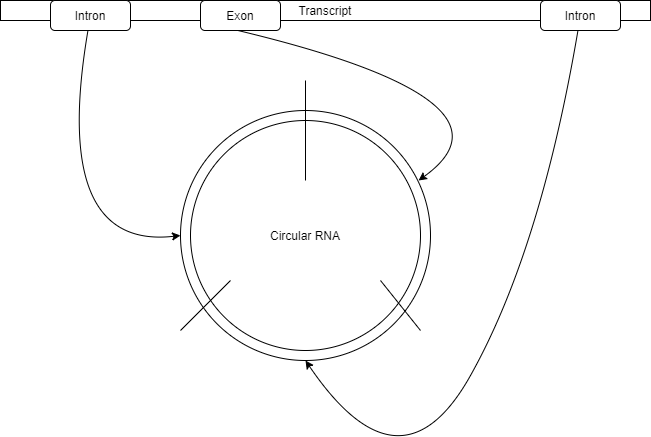
\includegraphics[width=8cm]{circ-rna}
	\caption{A demonstration of the formation of circular RNA from intron and exon biproducts of alternative splicing.
	}
	\label{fig:mesh1}
\end{figure}

\subsection{
\emph{Freq Analysis}} \label{s:conclusion}

    \begin{table}[!hbt]
      % Center the table
      \begin{center}
      % Fold Inductions
      \caption{QtPCR Fold Inductions}
      \label{tab:simParameters}
      % Table itself: here we have two columns which are centered and have lines to the left, right and in the middle: |c|c|
      \begin{tabular}{|c|c|}
        \hline
	  		# Region Types Intersected           & Frequency \\
        \hline
		1	& 14 \\
        \hline
		2	& 82 \\
        \hline
		3	& 20 \\
        \hline
		4	&  1 \\
        \hline

      \end{tabular}
      \end{center}
    \end{table}
	
	\subsection{
\emph{Freq Analysis}} \label{s:conclusion}

    \begin{table}[!hbt]
      % Center the table
      \begin{center}
      % Fold Inductions
      \caption{QtPCR Fold Inductions}
      \label{tab:simParameters}
      % Table itself: here we have two columns which are centered and have lines to the left, right and in the middle: |c|c|
      \begin{tabular}{|c|c|c|c|c|}
        \hline
		Database           & Version & Updated & Coordinate Format & Url \\
        \hline
		GWAS Catalog & NA & Frequently & hg38 & https://www.ebi.ac.uk/gwas/ \\
        \hline
		ClinVar & NA & Frequently & hg38 & https://www.ncbi.nlm.nih.gov/clinvar/ \\
        \hline
		Genecode & V37 & 02-2021 & hg38 & https://www.gencodegenes.org/ \\
        \hline
		RNACentral & NA & & hg19 & https://rnacentral.org/ \\
        \hline
		CircBase & 1.0 & 2017 & hg19 & http://www.circbase.org/ \\
        \hline
		SnoDB & 1.2.1 & Unknown & hg19 & http://scottgroup.med.usherbrooke.ca/snoDB/ \\
        \hline
		Eukaryotic Promoter Db & Unknown & 2019 & hg38 & https://epd.epfl.ch//index.php \\
        \hline
		Enhancer Atlas & 2.0 & Unknown & hg19 & http://www.enhanceratlas.org/ \\
        \hline
		CTCFBSDB & 2.0 & 2013 & hg19 & https://insulatordb.uthsc.edu/ \\
        \hline
      \end{tabular}
      \end{center}
    \end{table}



\end{document}